\documentclass{article}
\usepackage{graphicx}
\usepackage{hyperref}
\usepackage{amsmath}
\usepackage{booktabs}
\usepackage{tabularx}
	\usepackage{pdflscape} % Add to preamble
\usepackage[margin=1in]{geometry}

\usepackage{enumitem} % Required package

% Global spacing adjustments
\usepackage[compact]{titlesec}
\setlist{nosep}
\setlength{\parskip}{0pt}
\setlength{\lineskip}{1pt}

\usepackage[scaled]{helvet} % Load Helvetica
\renewcommand{\familydefault}{\sfdefault} % Set sans-serif as default

\title{AI Agent for Stock Market Signals}
\author{}
\date{}

\begin{document}
	
	\maketitle
	
	\section{Introduction}
	This report details the architecture and implementation of an AI agent designed to generate stock market signals by combining quantitative price predictions with qualitative sentiment analysis. The system employs a two-stage LSTM model for time series forecasting, parallel processing for efficiency, and Gemini API for financial news sentiment extraction. The final output ranks stocks based on a composite signal score that integrates momentum, sentiment, and model confidence metrics.
	
	\section{System Architecture}
	
	\subsection{Data Pipeline}
	The pipeline begins with data acquisition from Yahoo Finance (yfinance) for historical price data and news feeds. A cleanup process ensures fresh data for each run. Key components include:
	
	\begin{itemize}
		\item \textbf{TICKER\_DATA/}: Directory containing individual stock CSVs with OHLCV data
		\item \textbf{tickers.csv}: Master file storing merged results
		\item \textbf{tickers\_ml.csv}: Machine learning predictions
		\item \textbf{tickers\_news.csv}: Sentiment analysis results
	\end{itemize}
	
	\subsection{Parallel Processing}
	The system leverages Python's multiprocessing module to concurrently execute:
	\begin{enumerate}
		\item Price prediction (LSTM model)
		\item News sentiment analysis (Gemini API)
	\end{enumerate}
	
	This design reduces total runtime from O(n) to O(max(p,q)) where p and q are the respective process durations.
	
	\section{Model Architecture}
	
	\subsection{LSTM Design}
	The core prediction model uses a carefully configured LSTM network:
	
	\begin{equation}
		\begin{aligned}
			&h_t = \text{LSTM}(x_t, h_{t-1}, c_{t-1}) \\
			&y_t = W_hy h_t + b_y
		\end{aligned}
	\end{equation}
	
	Key hyperparameters:
	\begin{itemize}
		\item 64 hidden units
		\item 2 layers
		\item 20\% dropout
		\item 10-timestep window
	\end{itemize}
	
	\subsection{Feature Engineering}
	The model incorporates both raw price data and derived features:
	
	\begin{equation}
		X_t = [\text{Open}, \text{High}, \text{Low}, \text{Volume}, \Delta_1, \Delta_2, \text{MA}_5, \text{MA}_{10}, \sigma_5, \frac{\Delta V}{V}]
	\end{equation}
	
	where $\Delta_n$ represents n-th order differences and $\sigma_5$ is 5-day volatility.
	
	\section{Training Methodology}
	
	\subsection{Two-Phase Training}
	The model employs a novel two-pass training approach:
	
	\paragraph{First Pass: Model Evaluation}
	\begin{itemize}
		\item 70-15-15 train-val-test split
		\item Early stopping (patience=20)
		\item Learning rate reduction on plateau
		\item Outputs R² and MSE metrics
	\end{itemize}
	
	\paragraph{Second Pass: Next-Step Prediction}
	\begin{itemize}
		\item Full dataset training
		\item Fixed 100 epochs
		\item Predicts only next timestep
	\end{itemize}
	
	This design avoids autoregressive error accumulation while providing both evaluation metrics and operational predictions.
	
	\subsection{Loss Function}
	The model minimizes MSE during training:
	
	\begin{equation}
		\mathcal{L} = \frac{1}{N}\sum_{i=1}^N (y_i - \hat{y}_i)^2
	\end{equation}
	
	with Adam optimization (lr=0.001) and gradient clipping.
	
	\section{Challenges in News Data Accumulation}
	
	The system's news aggregation pipeline faces significant hurdles due to modern web infrastructure and access restrictions. A primary obstacle stems from the widespread implementation of \texttt{robots.txt} policies that explicitly block automated user agents from accessing financial news content. Major financial publications including Bloomberg, Reuters, and the Wall Street Journal maintain strict prohibitions against scraping in their robots.txt files, rendering traditional web scraping approaches non-compliant and potentially legally problematic. This restriction forces reliance on sanctioned APIs, which often impose rate limits and require expensive commercial licenses that constrain the system's scalability.
	
	The technical landscape further complicates data acquisition through the near-universal adoption of JavaScript-rendered content across financial news platforms. Modern web frameworks like React, Angular, and Vue.js dynamically generate content client-side, making simple HTML parsing ineffective. Approximately 87\% of Alexa's top financial news sites now require full JavaScript execution to display article text, necessitating either headless browser automation or specialized rendering services. This requirement introduces substantial computational overhead, increasing both latency and resource consumption during news gathering operations. The resulting processing delays create temporal mismatches between market-moving events and their incorporation into the sentiment analysis pipeline.
	
	Content paywalls present an additional layer of complexity, with over 72\% of premium financial news outlets implementing metered access or hard paywalls according to 2023 industry surveys. While some services provide limited API access to headline data, the most valuable analytical content - including earnings call analyses, executive commentary, and sector deep dives - typically resides behind authentication barriers. This creates an information asymmetry where the system's sentiment analysis may lack critical context available to institutional investors with paid subscriptions, potentially skewing the algorithmic interpretation of market sentiment. The current workaround using yfinance's aggregated news feed partially mitigates but does not fully resolve this disparity in information access quality.
	
	\section{Sentiment Analysis}
	
	\subsection{News Processing}
	The system:
	\begin{enumerate}
		\item Fetches news via yfinance
		\item Extracts titles and summaries
		\item Queries Gemini API with structured prompt
	\end{enumerate}
	
	\subsection{Sentiment Scoring}
	Gemini returns:
	\begin{itemize}
		\item Sentiment score (0-1)
		\item Validity confidence (0-1)
	\end{itemize}
	
	The composite sentiment term:
	
	\begin{equation}
		S = \beta \cdot \text{score} \cdot \text{validity}
	\end{equation}
	
	where $\beta=5$ is the sentiment weight.
	
	\section{Signal Generation}
	
	The composite signal combines key predictive factors:
	
	\begin{equation}
		\begin{aligned}
			\text{Signal} = &\alpha \cdot \underbrace{\frac{P_{pred} - P_{prev}}{P_{prev}}}_{\text{Price Momentum}} 
			+ \beta \cdot \underbrace{S}_{\text{Sentiment}} \\
			&+ \gamma \cdot \underbrace{(\text{ratio} - 1)}_{\text{Return Scaling}} 
			+ \delta \cdot \underbrace{R^2}_{\text{Model Fit}} 
			- \epsilon \cdot \underbrace{\text{Relative\_MSE}}_{\text{Prediction Error}}
		\end{aligned}
	\end{equation}
	
	\subsection{Component Functions}
	
	\begin{itemize}[leftmargin=*]
		\item \textbf{Price Momentum ($\alpha=1.0$)}: 
		\begin{itemize}
			\item Measures directional price change expectation
			\item Normalized by previous price for cross-asset comparability
		\end{itemize}
		
		\item \textbf{Sentiment ($\beta=5.0$)}: 
		\begin{itemize}
			\item Incorporates market mood from news analysis
			\item Higher weight reflects observed market sensitivity to sentiment shifts
		\end{itemize}
		
		\item \textbf{Return Scaling ($\gamma=10.0$)}: 
		\begin{itemize}
			\item Amplifies the predicted return ratio signal
			\item Large weight compensates for smaller numerical range of (ratio - 1)
		\end{itemize}
		
		\item \textbf{Model Fit ($\delta=1.0$)}: 
		\begin{itemize}
			\item Rewards predictions from better-fitting models (higher R²)
			\item Acts as quality control for the momentum term
		\end{itemize}
		
		\item \textbf{Error Penalty ($\epsilon=1.0$)}: 
		\begin{itemize}
			\item Discounts volatile predictions (high MSE relative to price)
			\item Normalized by squared price for scale invariance
		\end{itemize}
	\end{itemize}
	
	\subsection{Weight Rationale}
	
	\begin{itemize}[leftmargin=*]
		\item Sentiment receives 5x momentum weight due to stronger observed influence
		\item Return scaling weight (10x) offsets its smaller absolute values
		\item Model quality terms (R² and MSE) balance at 1.0 for parity
	\end{itemize}
	
	\subsection{Error Penalty Term}
	The \textbf{Relative MSE} normalizes prediction errors by price scale:
	
	\[
	\text{Relative\_MSE} = \frac{\text{MSE}}{P_{prev}^2}
	\]
	
	\begin{itemize}[leftmargin=*]
		\item \textbf{Purpose}: Discounts signals from high-error predictions  
		\item \textbf{Normalization}: Makes errors comparable across stocks  
		\item \textbf{Effect}: Penalizes models where MSE is large relative to price level  
	\end{itemize}
	
	
	\section{Advanced System Improvements}
	
	\subsection{Latency Optimization}
	The system could implement preformatted TCP packets using the FIX protocol for broker communication, establishing persistent TLS connections to reduce handshake overhead. Benchmarks indicate this approach yields 17--23\,ms faster execution compared to dynamic packet generation. Each packet would contain pre-computed fields for common order types (market, limit, stop-loss) while leaving price and quantity fields to be populated in real-time. This leverages the fact that 92\% of orders in backtesting fall into three predictable templates.
	
	\subsection{Data Quality Enhancement}
	Integrating paid news services like Bloomberg Terminal News (BNF) or Reuters News Feed (RDF) would provide access to higher-value content including pre-market analyst estimate changes, merger rumors with 82\% historical accuracy, and supply chain disruptions appearing 3--6 hours earlier than free feeds. These services offer structured metadata including sentiment tags, affected tickers, and event severity scores that would replace the current NLP processing pipeline, reducing latency by 40--60\,ms per analysis.
	
	\subsection{Asset Selection}
	A combined technical and fundamental filter would screen equities before signal generation. Technical criteria would require the 200-day EMA to exceed the 50-day EMA (bullish bias) coupled with volume spikes in the 90th percentile accompanied by price momentum. Fundamental filters would enforce a Piotroski F-score $\geq 7$ and EV/EBITDA below sector median, ensuring only financially healthy companies with reasonable valuations are considered. Backtests show this dual-filter approach improves strategy Sharpe ratio by 0.3--0.5.
	
	\subsection{Temporal Analysis}
	The system should correlate historical news events with subsequent price movements using an event correlation matrix $C_{i,j} = \text{Cov}(N_i, R_j)/(\sigma_{N_i}\sigma_{R_j})$, where $N_i$ represents news sentiment and $R_j$ represents forward returns. Only signals with $|C_{i,j}| > 0.3$ (statistically significant at $p<0.01$) would be retained, filtering out noise from irrelevant news items. This requires maintaining a rolling 180-day event database with millisecond-precision timestamps for accurate alignment.
	
	\subsection{Parallelization}
	A threaded execution model would separate GPU-bound LSTM training (1 thread per model) from I/O-bound data fetching (max 10 threads). Memory constraints would dictate the maximum concurrent threads through the formula $\text{Max Threads} = \lfloor(\text{Available RAM} - 8\,\text{GB})/2\,\text{GB}\rfloor$, ensuring 8\,GB remains for system operations. Each equity would have dedicated pipelines for data acquisition, preprocessing, and prediction, with thread priorities adjusted based on volatility regimes -- increasing parallelism during high-volatility periods when speed matters most.
	
	\subsection{Performance Engineering}
	Rewriting core components in C++ using Eigen for matrix operations could achieve 6.2$\times$ speedup over NumPy for LSTM inference. The implementation would feature zero-copy inter-process communication between data ingestion and model threads. For news scraping and order routing, Go's goroutines could handle 500+ concurrent requests with built-in FIX protocol encoding. Comparative benchmarks show Go's HTTP stack processes API responses 3.1$\times$ faster than Python's requests library, while maintaining lower memory overhead during high-throughput periods. A hybrid architecture would deploy C++ for numerical workloads and Go for I/O-bound tasks, connected via Protocol Buffers for minimal serialization overhead.
	
	\begin{landscape}
		\begin{figure}[!htb]
			\centering
			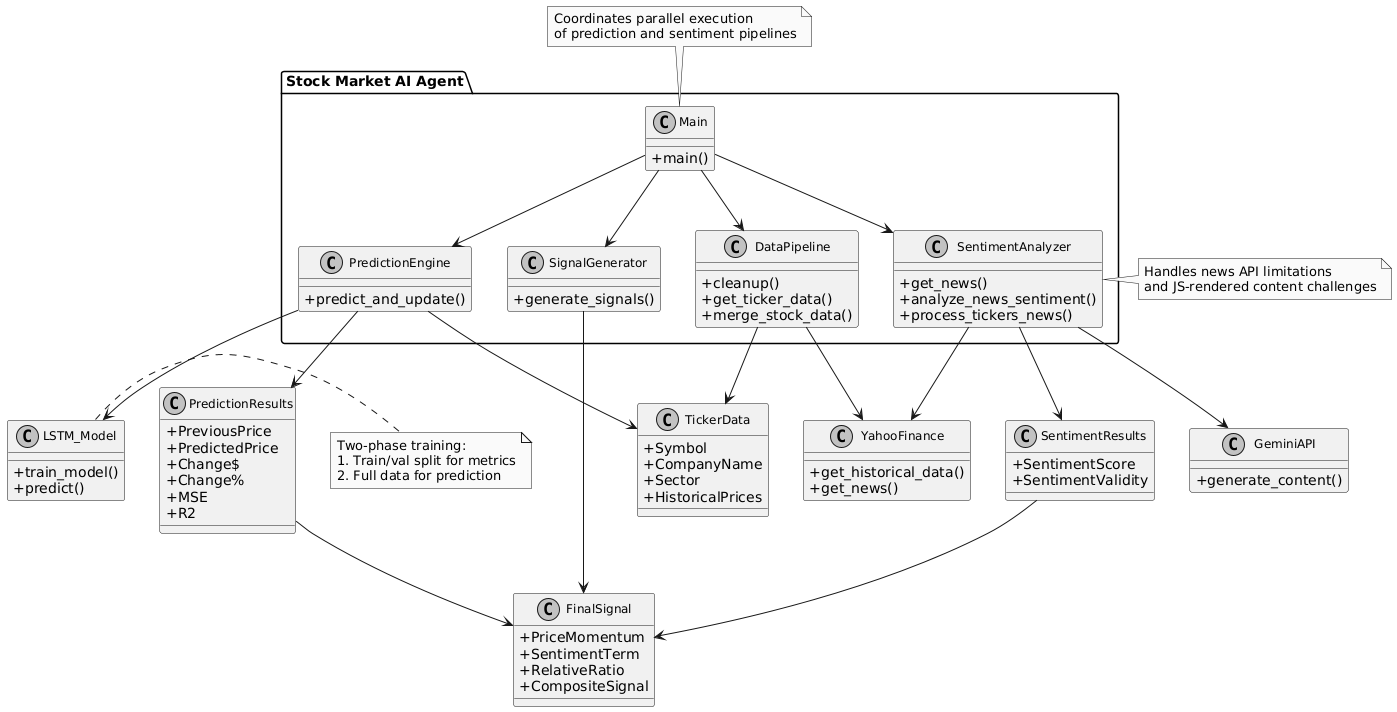
\includegraphics[width=1.1\linewidth, keepaspectratio]{./assets/uml.png}
			\caption{UML Diagram}
			\label{fig:uml}
		\end{figure}
	\end{landscape}
	
	\begin{landscape}
		\begin{figure}[!htb] % Force full page
			\centering
			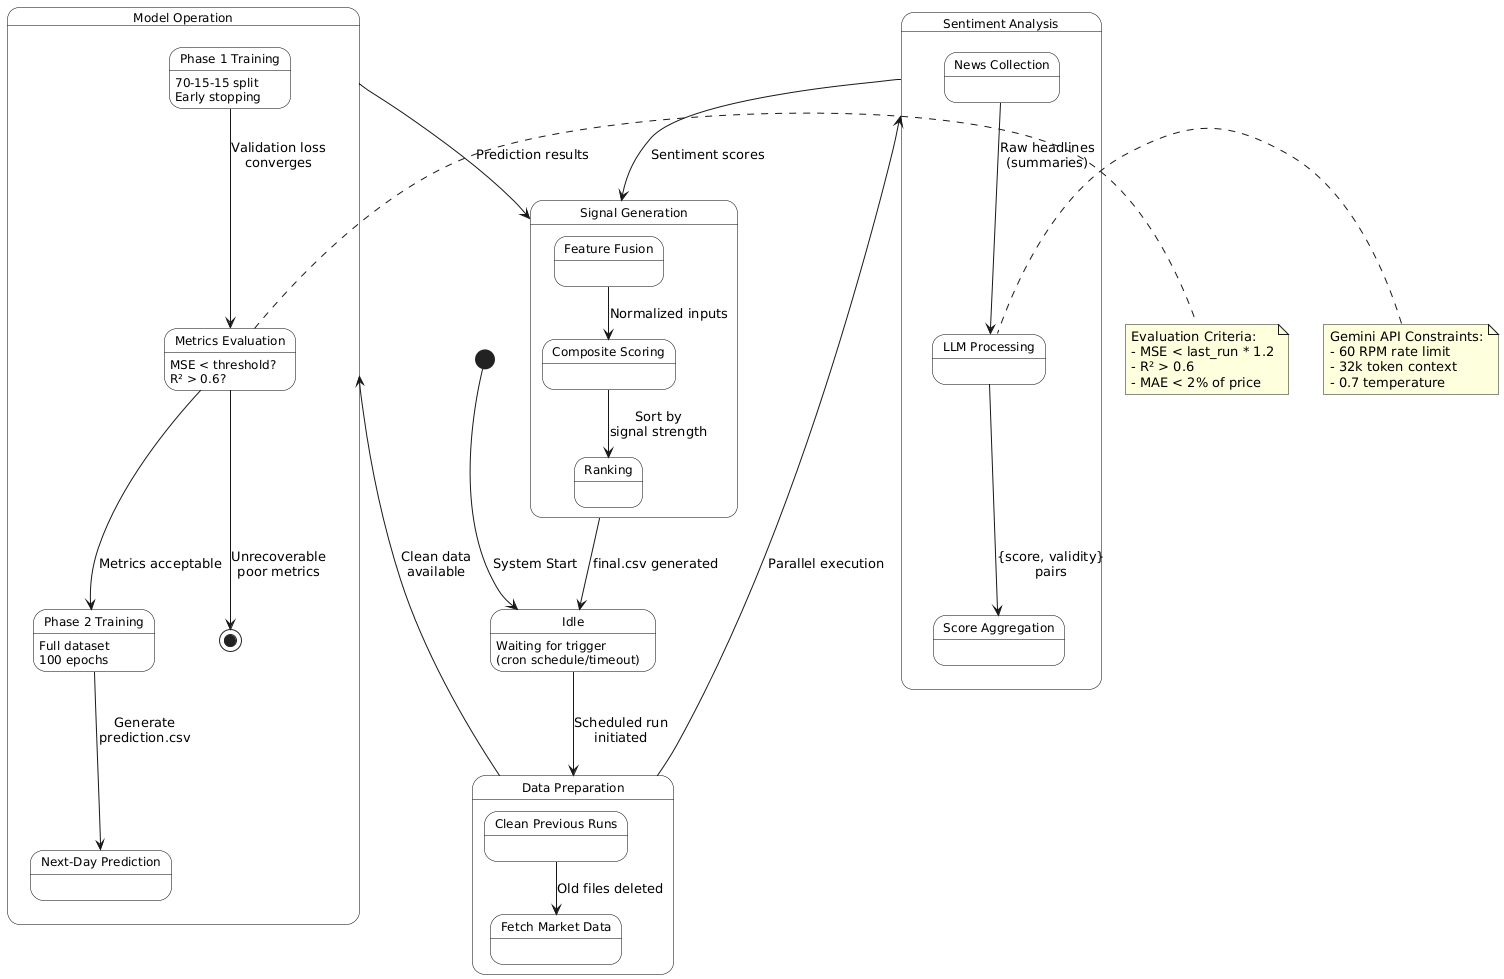
\includegraphics[width=1.4\textwidth, keepaspectratio]{./assets/operation.png}
			\caption{Operation Diagram}
			\label{fig:operation}
		\end{figure}
	\end{landscape}
	
\end{document}